~
\newpage
\section*{Appendix}
\addcontentsline{toc}{section}{Appendix}

\subsection*{A.1\quad Appendix to Chapter 1: An Introduction to Climate Change}

\begin{minipage}{\textwidth}
    \captionof{figure}{Contemporary Climate Models are Highly Accurate \label{cmip6_accuracy}}
    \centering
    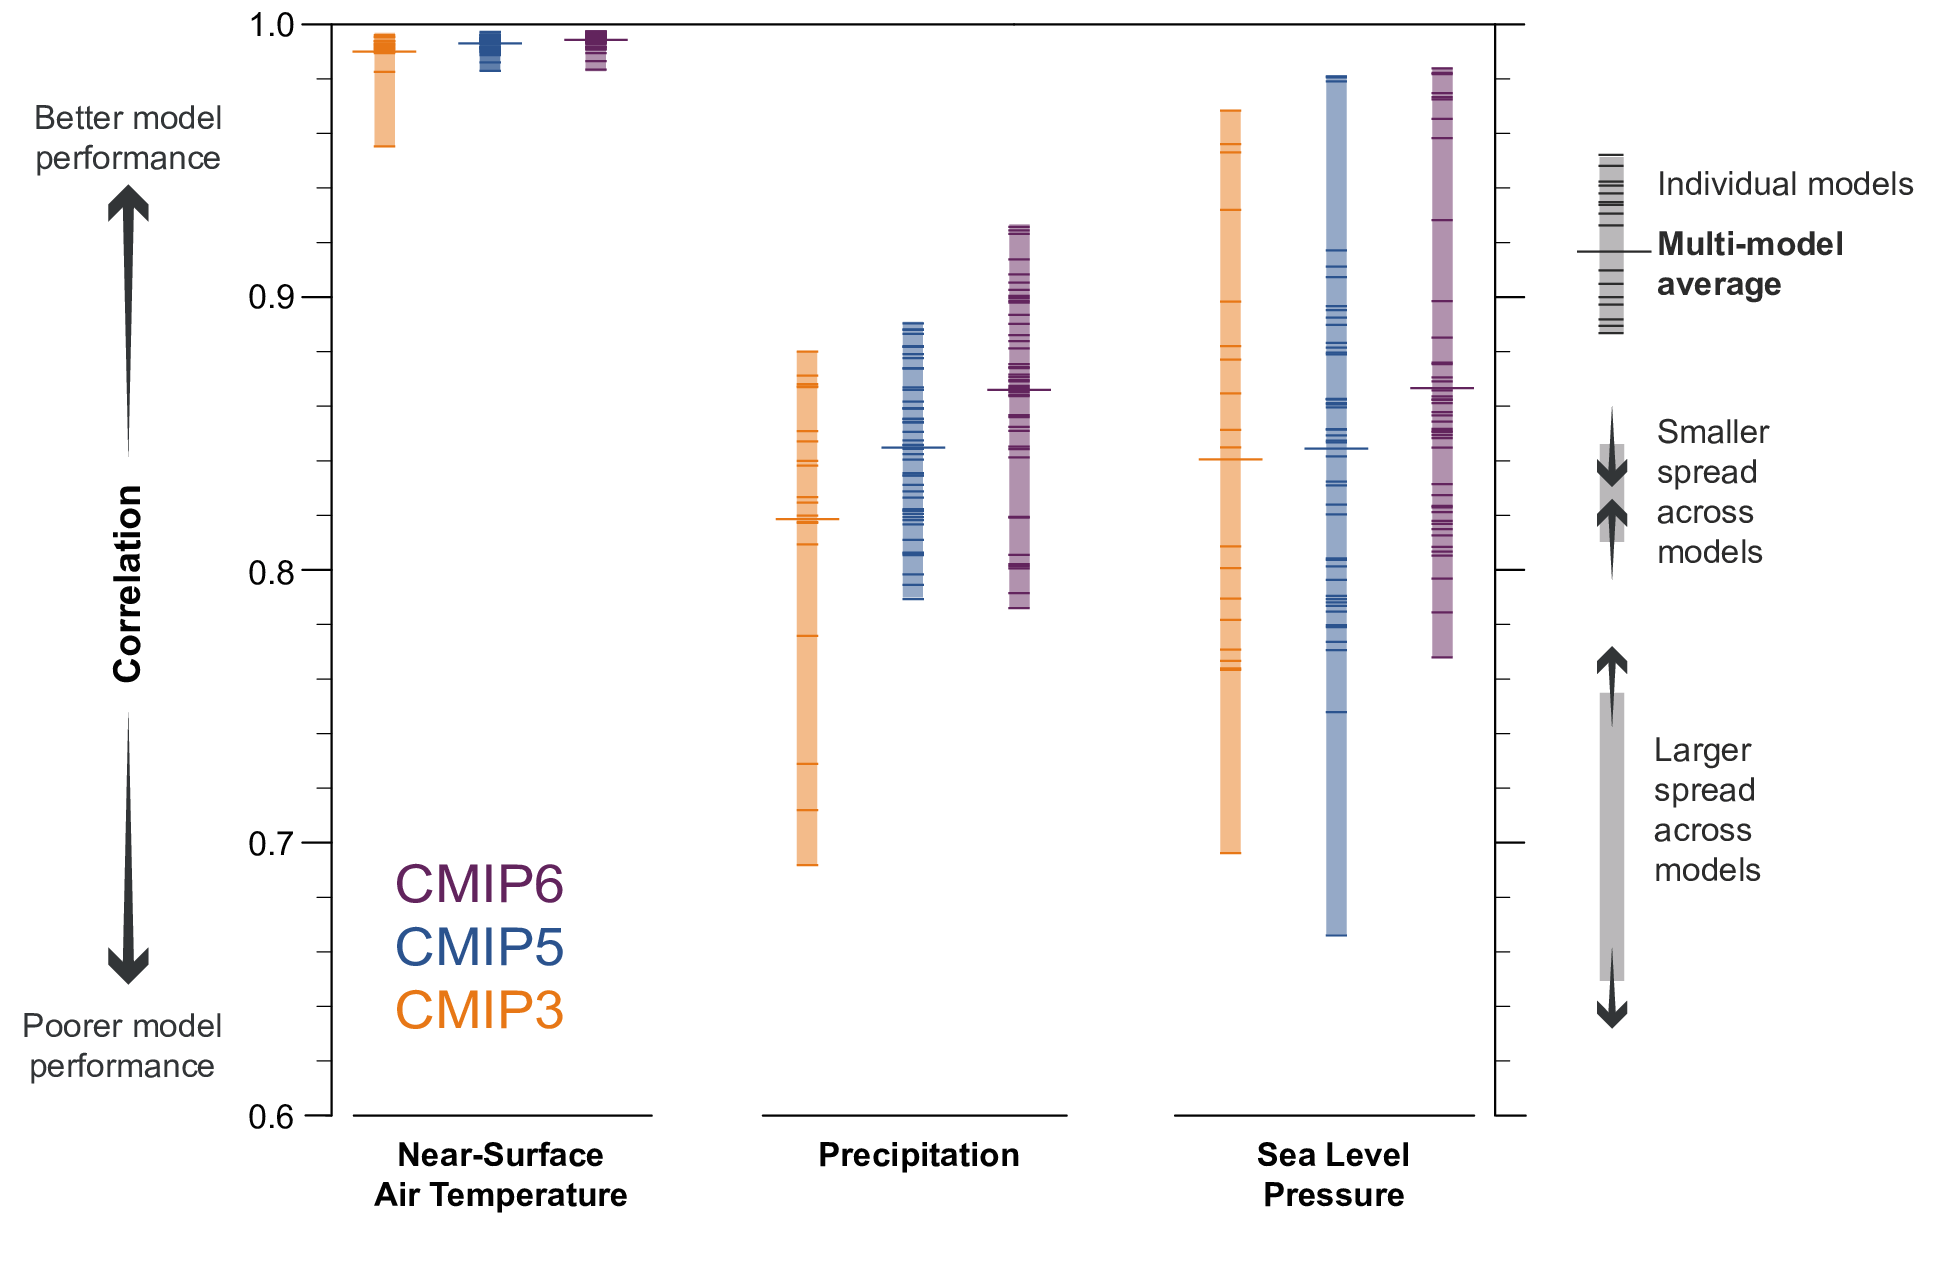
\includegraphics[width=0.7\textwidth]{figures/chapter1_figures/climate_model_accuracy.png}
    \fignote[1]{Figure from \cite{ipccAR6_model_accuracy}. The figure displays predictions for three common climate variables, near-surface air temperature, precipitation, and sea level pressure, under three different climate models. These three models are the Coupled Model Intercomparison Project Phases 3, 5, and 6. These are the three climate models used in the IPCC's fourth, fifth, and sixth assessment reports. There is no CMIP4 due to re-numbering. The vertical axis is the correlation between the model predicted outcomes the actual, observed outcomes. Clearly these models can predict near-surface air temperatures with near perfect accuracy. Other climate variables, like precipitation and sea levels rise have been more difficult to predict, but are still reasonably accurate. Climate scientists continue to learn more about the physical processes underlying climate, and consequently, these models continue to improve.
    }
\end{minipage}

\newpage
\subsection*{A.2\quad Appendix to Chapter 2: Designing Climate Policy}

\subsubsection*{The Environmental Kuznets Curve}

The contemporary literature on the relationship between economic standard of living and environmental decay begins with Simon Kuznets, and his work related not to the environment, but inequality. \cite{kuznets1955economic} laid out a empirical relationship between economic development and inequality. Kuznets findings suggest that income inequality rises as countries move from low-income to middle-income, and income inequality falls as countries move from middle-income to high-income. Diagrammatically, this creates an inverted U-shaped path called the Kuznets Curve with GDP per capita on the horizontal axis and measures of inequality (usually the income ratio between the top quintile and bottom quintile of earners) on the vertical axis. Realizing that economic development and environmental degradation follow a similar relationship, \cite{NBERw3914} were the first to formulate the \emph{Environmental} Kuznets Curve (EKC) in an analysis of NAFTA. While the model was not the primary focus of the original paper, it later led to its own published paper, \cite{grossman1995economic} and is now a standard in environmental economics. 

Figure \ref{EKC} displays the Environmental Kuznets Curve. The EKC hypothesizes that low-income economies will have relatively high environmental quality, as these economies may be more agrarian or pastoral. Countries often move from low-income to middle-income through industrialization, and as countries industrialize, their environmental degradation increases. Eventually though, economic development requires countries to move away from manufacturing and into higher human capital industries. When this happens, sectors dependent on high human capital (e.g., finance, engineering, education) tend to be less harsh on the environment. Past the turning point, economic development will decrease environmental degradation. 

\begin{figure}
\centering
\begin{minipage}{0.48 \textwidth}
\caption{The EKC \label{EKC}}
\begin{tikzpicture}[scale = 0.6]
\draw[thick, <->] (0,10) -- (0,0) -- (10,0);
\draw[thick, color1]  [domain = 1:9] plot (\x, {8.5 - .5*(\x - 5)^2});
\node [below right] at (7,0) {GDP/Capita};
\node[rotate=90, above] at (0,7) {Environmental Degradation};
\draw[dashed] (5,0) -- (5,9.5) node[right]{\footnotesize Turning Point};
\end{tikzpicture}
\end{minipage}
\begin{minipage}{0.48\textwidth}
\centering 
\caption{Application of the  EKC}
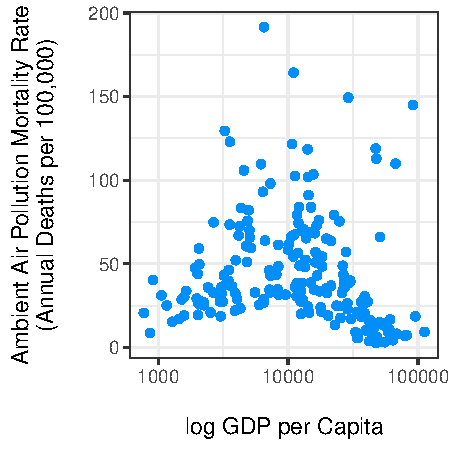
\includegraphics[width=0.9\textwidth]{figures/chapter2_figures/ekc.pdf}
\end{minipage}
Data from \cite{owidoutdoorairpollution} 
%https://ourworldindata.org/outdoor-air-pollution#outdoor-air-pollution-tends-to-rise-with-industrialization-before-falling
\end{figure}

Despite its quick adoption in the discipline and its continued use, the EKC has largely been discredited \citep{stern2004rise}. \cite{arrow1995economic} importantly note that the usual form of the EKC does not allow for any feedback between the environment and development, implicitly assuming that pollution and other forms of environmental degradation do not hinder economic development. 

\newpage
\subsection*{A.3\quad Appendix to Chapter 3: Ambient Air Pollution \& Electricity Generation}



\newpage
\subsection*{A.4\quad Appendix to Chapter 4: A Model of Emissions Pricing \& Environmental Inequality}

\begin{center}
    \singlespacing
    \renewcommand{\arraystretch}{1.5}
    \captionof{table}{Overview of Notation\label{notation}}
    \small
\begin{longtable}{c L{0.55\textwidth} C{0.15\textwidth} c}
    \hline\hline 
    Variable & Description & Determined & Source\\
    \hline \\[-1.8ex]
    \multicolumn{4}{l}{\emph{Indices \& Model Environment}}\\
    \hline 
    $i$ & Generator identifier & -- & -- \\
    $r$ & Region identifier & -- & -- \\
    $\ell$ & Transmission line identifier & -- & -- \\
    $m$ & Subregion or community identifier & -- & --\\ 
    $N$ & The number of generators & Exogenous & (1) \\
    $\mathcal{N}$ & Set of all generators; $\mathcal{N} = \{1, \ldots, N\}$ & Exogenous & (1) \\
    $\mathcal{N}_r$ & Set of all generators in region $r$ & Exogenous &  (1) \\
    $R$ & The number of regions & Exogenous &  (1) \\
    $\mathcal{L}$ & Set of all transmission lines & Exogenous &  (5) \\
    $M$ & Number of subregions or communities & Exogenous &  (3), (4)\\
    $T$ & Final period of the generation phase & Exogenous &  Chosen\\
    \\[-1.8ex]
    \multicolumn{4}{l}{\emph{Investment Phase}}\\
    \hline 
    $\mathcal{J}$ & Set of all investment options & Exogenous & Chosen\\
    $j_i$ & Generator $i$'s investment decision; $j_i \in \mathcal{J}$ & Endogenous & -- \\
    $j$ & Investment profile, $j = (j_1, j_2, \ldots, j_N)$ & Endogenous & -- \\
    $\rho_i^0$ & Generator $i$'s initial heat rate (BTU/kWh) & Exogenous & (1) \\
    $\rho_i$ & Generator $i$'s heat rate (BTU/kwh) & Endogenous & -- \\
    $\tilde{\delta}$ & Heat rate depreciation rate from the investment phase to the generation phase; $\tilde{\delta} \in (0, 1)$ & Exogenous & (10) \\
    $v_i$ & Generator $i$'s stochastic investment cost shock; $v_i > 0$ for all $i \in \mathcal{N}$ & Exogenous & Chosen \\
    $\gamma$ & Constant scalar in the investment cost function; $\gamma > 0$ & Exogenous & \\
    $\alpha$ & Scale parameter in the investment cost function; $\alpha > 0$ & Exogenous & \\
    $\Gamma (j_i, v_i)$ & Investment costs for generator $i$; a function of generator $i$'s investment choice $j_i$ and $i$' stochastic investment cost shock $v_i$ & Endogenous & -- \\
    $\Gamma (j \mid v)$ & Total investment costs for all generators; a function of the investment profile $j$ given a vector of all generator's stochastic investment cost shocks $v$ & Endogenous & -- \\
    $Q_t^e$ & $R$-dimensional vector of expected quantities demanded of electricity at time $t$ for each region (kWh) & Exogenous & (2)\\
    \\[-1.8ex]
    \multicolumn{4}{l}{\emph{Generation Phase}}\\
    \hline 
    $a_{it}$ & Operating decision of generator $i$ in period $t$; $a_{it} \in \{0, 1, \ldots, R\}$ where $a_{it} = r$ indicates that generator $i$ operates in period $t$ to sell its generation in region $r$ and $a_{it} = 0$ indicates that generator $i$ does not operate in period $t$ & Endogenous & -- \\
    $a_t$ & Profile of operating decisions in period $t$; $a_t = (a_{1t}, a_{2t}, \ldots, a_{Nt})$ & Endogenous & -- \\
    $\overline{q}_i$ & Generator $i$'s nameplate capacity (kW); the maximum rated generation of generator $i$ in an hour & Exogenous & (1) \\
    $q_{itr}$ & Generator $i$'s generation to be sold in region $r$'s wholesale electricity market at time $t$ (kWh) & Endogenous & -- \\
    $f_i$ & The primary fuel type of generator $i$; $f_i \in \{\text{Coal}, \text{Natural Gas}, \text{Oil}\}$ & Exogenous &  (1) \\
    $u_{f_i}$ & Unit cost of generator $i$'s fuel $f_i$ (\$/BTU) & Exogenous & (6), (7), (8)\\

    $e_{f_i}$ & Greenhouse gas emissions intensity of generator $i$'s fuel $f_i$ (tonnes CO$_2$e/BTU) & Exogenous & \\

    $\tau_r$ & Greenhouse gas emissions tax in region $r$ (\$/tonnes CO$_2$e) & Exogenous & (9) \\
    $P_{tr}$ & Price of electricity in region $r$'s wholesale market at time $t$ & Endogenous & -- \\
    $Q_{tr}$ & Quantity of electricity demanded in region $r$'s wholesale market at time $t$ & Exogenous &  (2) \\
    $C(a_t\mid j)$ & Total cost of generation in period $t$; a function of the profile if operating decisions $a_t$ given the profile of investment decisions $j$ & Endogenous & -- \\
    $MC(j)$ & Marginal cost matrix, $N \times R$; a function of the investment profile (vector) $j$; element in the $i$th row and $r$th column is $mc_{ir}$ & Endogenous & -- \\
    $G(a_t)$ & Generation matrix, $N \times R$; a function of the operating decision profile (vector) $a_t$; element in the $i$th row and $r$th column is $q_{itr}$ or $\overline{q}_i \1(a_{it} = r)$ & Endogenous & --\\
    $\rho^0$ & $N$-dimensional vector of heat rates in the absence of investment; the $i$th element is $\rho_i^0(1 + \tilde{\delta})$ & Endogenous & -- \\
    $D_{\rho^0 - j}$ & Diagonalized $N\times N$ matrix corresponding with the vector $\rho^0 - j$; for elements along the diagonal, the element in the $i$th row and $i$ column is $\rho_i = \rho_i^0(1 + \tilde{\delta}) - j_i$, all elements not along the diagonal are 0 & Endogenous & -- \\
    $U$ & Unit cost matrix, $N\times R$; the element in the $i$th row and $r$th column is generator $i$'s cost in region $r$ per BTU, $u_{f_i} + e_{f_i}\tau_r$ & Derived & -- \\
    $\overline{q}$ & $N$-dimensional vector of nameplate capacities; $\overline{q} = (\overline{q}_1, \overline{q}_2, \ldots, \overline{q}_N)$ & Derived & -- \\
    $D_{\overline{q}}$ & Diagonalized $N\times N$ matrix corresponding with the vector $\overline{q}$; for elements along the diagonal, the element in the $i$th row and $i$th column is $\overline{q}_i$, all elements not along the diagonal are 0 & Derived & -- \\
    $\1(a_t)$ & Operating decisions matrix, $N \times R$; the element in the $i$th row and $r$th column is $\1(a_{it} = r)$ & Endogenous & -- \\
    $\delta$ & Hourly discount factor, $\delta \in (0, 1)$ & Exogenous & (10)\\
    $y_{tr}$ & Net electricity exports for region $r$ at time $t$; alternatively, understood as a marginal power injection out of region $r$ at time $t$ & Endogenous & -- \\
    $PTDF_{r\ell}$ & Power transfer distribution factor on transmission line $\ell$ out of region $r$ & Exogenous & (5)\\
    $\text{Cap}_\ell$ & Maximum capacity of transmission line $\ell$ (kW) & Exogenous & (5)\\
    \\[-1.8ex]
    \multicolumn{4}{l}{\emph{The EI Gap}}\\
    \hline 
    $d$ & $M$-dimensional vector of communities' disadvantaged status; the $m$th element is 1 is $m$ is a disadvantaged community and 0 otherwise & Exogenous & (3), (4)\\
    $w$ & Local air pollutant identifier & -- & -- \\
    $e_i^w$ & Generator $i$'s emissions intensity of air pollutant $w$ (pounds/kWh) & Exogenous & (1)\\
    $w_{it}$ & Generator $i$'s emissions of air pollutant $w$ (lbs) & Endogenous & -- \\
    $\phi_w(w_{it}\mid i, t)$ & $M$-dimensional vector of the changes in the concentration of air pollutant $w$ across all $M$ communities resulting from $w_{it}$, the emissions of air pollutant $w$ from generator $i$ in time $t$ & Endogenous & -- \\
    $\Phi_w^1(T)$ & Average change in the concentration of pollutant $w$ for disadvantaged communities (elements of $d$ equal to 1) after $T$ periods & Endogenous & -- \\
    $\Phi_w^0(T)$ & Average change in the concentration of pollutant $w$ for non-disadvantaged communities (elements of $d$ equal to 0) after $T$ periods & Endogenous & -- \\
    $\text{EIGap}_w(T)$ & The environmental inequality gap after $T$ periods & Endogenous & -- \\
    \hline\hline
\end{longtable}
\fignote[1]{Table summarizes the notation used in Chapter 4. In general, lowercase letters without an index are profiles/vectors, plain-text uppercase letters denote matrices or the size of a set, and uppercase letters in the \texttt{mathcal} font are sets (e.g., $\mathcal{N}$). We denote the equilibrium of any variable as the variable with an asterisk. Derived variables are those that are a deterministic function of entirely exogenous variables. The source key for exogenous variables correspond with the data sources in Table \ref{data_sources}.}
\end{center}


\begin{center}
    \singlespacing
    \renewcommand{\arraystretch}{1.5}
    \captionof{table}{Data Sources Key\label{data_sources}}
    \small
    \begin{longtable}{c L{0.8\textwidth}}
        \hline\hline
        Source Key & Source Citation\\
        \hline \\[-3ex]
        (1) & United States Environmental Protection Agency (EPA). 2021. ``Emissions \& Generation Resource Integrated Database (eGRID), 2019" Washington, DC: Office of Atmospheric Protection, Clean Air Markets Division. Available from EPA's eGRID web site: \url{https://www.epa.gov/egrid}.\\ \\[-3ex]
        \hline \\[-3ex]
        (2) & United States Energy Information Administration (EIA). 2023. ``Hourly Electric Good Monitor'' Region Files. Available at: \url{https://www.eia.gov/electricity/gridmonitor/dashboard/electric_overview/US48/US48}\\ \\[-3ex]
        \hline \\[-3ex]
        (3) & United States Environmental Protection Agency. 2021 version. EJScreen. Census Tract-Level US Percentiles. Retrieved: 2023-03-03. Available at: \url{https://gaftp.epa.gov/EJSCREEN/2021/} \\ \\[-3ex]
        \hline \\[-3ex]
        (4) & California Office of Environmental Health \& Hazard Assessment (OEHHA). 2022. SB 535 Disadvantaged Communities. Retrieved: 2023-03-03. Available at: \url{https://oehha.ca.gov/calenviroscreen/sb535} \\ \\[-3ex]
        \hline \\[-3ex]
        (5) & Fowlie, Meredith, Petersen, Claire, and Reguant, Mar. Data and Code for: Border Carbon Adjustments When Carbon Intensity Varies Across Producers: Evidence from California. Nashville, TN: American Economic Association [publisher], 2022. Ann Arbor, MI: Inter-university Consortium for Political and Social Research [distributor], 2021-05-13. \url{https://doi.org/10.3886/E131024V1} \\ \\[-3ex]
        \hline \\[-3ex]
        (6) & United States Energy Information Administration. 2023. Natural Gas Electric Power Price. Source key: N3045. Available at: \url{http://www.eia.gov/dnav/ng/ng_pri_sum_a_epg0_peu_dmcf_m.htm} \\ \\[-3ex]
        \hline \\[-3ex]
        (7) & United States Energy Information Administration. 2023. Coal shipments to the electric power sector: price, by plant state. Available at: \url{https://www.eia.gov/coal/data/browser/} \\ \\[-3ex]
        \hline \\[-3ex]
        (8) & United States Energy Information Administration. 2023. Cushing, OK WTI Spot Price FOB (Dollars per Barrel). Source key: RWTC. Available at: \url{https://www.eia.gov/dnav/pet/hist/LeafHandler.ashx?n=PET&s=RWTC&f=M} \\ \\[-3ex]
        \hline \\[-3ex]
        (9) & California Air Resources Board. 2023. Cap-and-Trade Program Data Dashboard---Carbon Allowance Prices. Available at: \url{https://ww2.arb.ca.gov/our-work/programs/cap-and-trade-program/program-data/cap-and-trade-program-data-dashboard} \\ \\[-3ex]
        \hline \\[-3ex]
        (10) & Board of Governors of the Federal Reserve System (US), Market Yield on U.S. Treasury Securities at 10-Year Constant Maturity, Quoted on an Investment Basis [DGS10]. Retrieved: 2023-03-03 from FRED, Federal Reserve Bank of St. Louis. Available at: \url{https://fred.stlouisfed.org/series/DGS10} \\ \\[-3ex]
        \hline \\[-3ex]
        (11) & United States Energy Information Administration. 2022. Carbon Dioxide Emissions Coefficient. Available at: \url{https://www.eia.gov/environment/emissions/co2_vol_mass.php}\\ \\[-3ex]
        \hline\hline
    \end{longtable}
\end{center}

\newpage
\subsection*{A.5\quad Appendix to Chapter 5: Carbon Pricing \& Air Pollution Disparities in California}
